\documentclass[letterpaper,openany,twoside,twocolumn]{book}

\newcommand{\PATH}{../../../}

\usepackage[justified]{\PATH dndtemplate/dnd}

\usepackage{\PATH regions/stylesheets/monster_book_commands}
\usepackage{\PATH regions/stylesheets/regions_stylesheet}
\usepackage{\PATH regions/stylesheets/dungeon_stylesheet}
\usepackage{\PATH regions/stylesheets/monster_stylesheet}
\usepackage{\PATH regions/stylesheets/shadowfy}

\usepackage[english]{babel}
\usepackage[utf8]{inputenc}

%\newcommand{\entryfont}{\DndFontStatBlockBody} & uses the default font provided by the LaTeX DnD-Template
\newfontfamily\entryfont{Kalam}[Path=\PATH template/fonts/,Extension=.ttf,UprightFont=Kalam-Regular,BoldFont=Kalam-Bold] % requires XeLaTeX or LuaTeX
\newfontfamily\titlefont{Modesto Bold(2)}[Path=\PATH template/fonts/,Extension=.otf,UprightFont=Modesto Bold(2),BoldFont=Modesto Bold(2)] % requires XeLaTeX or LuaTeX

\begin{document}
	% Titlepage	
	\monstersTitlePage{Mossdrip Caverns}{images/titlepage_Mossdrip_Caverns.jpg}{0.5cm}{0cm}{height=\paperheight}{https://wallpapersden.com/tomb-castle-ladder-wallpaper/}{Ancient Tomb}{WallpapersDen}{A collection of homebrew monsters found in the Mossdrip Caverns}
	
	\tableofcontents
	
	\mainmatter
	
	\graphicspath{{./images},{./monsters/Fleshgorger_Ant/images}}

\MonsterSheetGeometry

% --------------------------------------------------------------------------------------------------- %
% ################################################################################################### %
% #-#-#-#-#-#-#-#-#-#-#-#-#-#-# Monster-Sheet with two Smaller Pictures #-#-#-#-#-#-#-#-#-#-#-#-#-#-# %
% ################################################################################################### %
% --------------------------------------------------------------------------------------------------- %

\chapter*{Giant Fleshgorger Ant}
\stepcounter{chapter}
\addcontentsline{toc}{chapter}{\protect\numberline{\thechapter}Giant Fleshgorger Ant}
\vspace*{-3\fontdimen6\font}

\entryfont \noindent \DndDropCapLine{P}robably the most common swarm-dwelling vermin, ant colonies reside in massive mounds creating a giant network of tunnels and caves. The Giant Fleshgorger Ant is a very vicious and aggressive type which change the whole area wherever they settle down. Fitting to their name they feed on other species,  most often carrions but they are also fitted for hunting. There exist not a lot of species that can withstand an onslaught of hungry a Fleshgorger Ant colony.
\vspace*{6cm}
	
\MonsterGraphicAndShortInfo{shortinfo}% shortinfo or none for no Short-Info Box
{%
	{1.5cm}% Shift Horizontal Short Info Box
	{3.5cm}% Shift Vertical Short Info Box
	{0}% Rotation Angle Short Info Box
	{3.5cm}% Width of Short-Info Box
	{5}% Number of Lines in Textbox (might be adjusted after 1 compile) 
	{%
		The Giant Fleshgorger Ant should not be underestimated as its strength and aggressiveness exceed even those of much larger species.%
	}%
}%
{1cm}% Shift Horizontal Monster Graphic
{-5.75cm}% Shift Vertical Monster Graphic
{, anchor=north west}% Further Picture Placement Options
{(current page.north west)}% Anchor-Point on Page
{height=275pt}% Dimension of Graphic
{Worker_Ant.png}%
\addImageDBEntry{FleshgorgerAnt1}{Page \thepage}{Art}{https://scryfall.com/card/tmid/9/insect}{Insect Token MtG Art from Innistrad: Midnight Hunt}{Nicholas Gregory}%
	
\begin{DndMonster}[width=0.5\textwidth]{Fleshgorger Worker Ant}
    \DndMonsterType{Medium Monster, unaligned}

    % If you want to use commas in the key values, enclose the values in braces.
    \DndMonsterBasics[
        armor-class = {10 (Natural Armor)},
        hit-points  = {\DndDice{2d8+6}},
        speed       = {30 ft., burrow 25 ft., climb 25 ft.},
    ]

    \DndMonsterAbilityScores[
        str = 14,
        dex = 10,
        con = 17,
        int = 1,
        wis = 12,
        cha = 11,
    ]

    \DndMonsterDetails[
        %saving-throws = {Str +0, Dex +0, Con +0, Int +0, Wis +0, Cha +0},
        skills = {Acrobatics +6, Perception +3},
        %damage-vulnerabilities = {cold},
        %damage-resistances = {bludgeoning, piercing, and slashing from nonmagical attacks},
        %damage-immunities = {cold},
        senses = {blindsight 30ft., passive Perception 13},
        %condition-immunities = {frightened, poisoned},
        %languages = {-},
        challenge = 1,
    ]
    
    \DndMonsterAction{Powerful Build}
    The ant counts as one size larger for the purpose of determining its carrying capacity, the weight it can push, drag, or lift, and creatures it can grapple.
    
    \DndMonsterAction{Insect Climb}
    The ant can climb difficult surfaces without the need of performing ability checks.
    
    \DndMonsterAction{Hive Tactics}
    The ant has advantage on attack roles on creatures within 5 ft. of one of the ant's allies.
    
    \DndMonsterAction{Hive Mind}
    The ant is immune to being charmed or frightened.
	
	\DndMonsterSection{Actions}
	\DndMonsterAction{Multiattack}
	The Fleshgorger Ant can make a Bite Attack and a Sting Attack on its turn.
	
	\DndMonsterAttack[
      name=Bite,
      distance=melee, % valid options are in the set {both,melee,ranged},
      %type=weapon, %valid options are in the set {weapon,spell}
      mod=+4,
      reach=5,
      %range=20/60,
      targets=one target,
      dmg=\DndDice{1d8 + 2},
      dmg-type=piercing,
      %plus-dmg=,
      %plus-dmg-type=,
      %or-dmg=,
      %or-dmg-when=,
      %extra=,
    ]
    
    \DndMonsterAttack[
      name=Sting,
      distance=melee, % valid options are in the set {both,melee,ranged},
      %type=weapon, %valid options are in the set {weapon,spell}
      mod=+4,
      reach=5,
      %range=20/60,
      targets=one target,
      dmg=\DndDice{1d4 + 2},
      dmg-type=piercing,
      %plus-dmg=,
      %plus-dmg-type=,
      %or-dmg=,
      %or-dmg-when=,
      extra={. Creatures must succed a DC 13 Constitution Saving Throw or take \DndDice{2d6} poison damage. On a successful save, it takes half damage},
    ]
      
\end{DndMonster}

\vfill\eject % cammand to break to next column
\vspace*{-3cm}%
\begin{center}\begin{tikzpicture}%
	\node (picture) at (0,0) {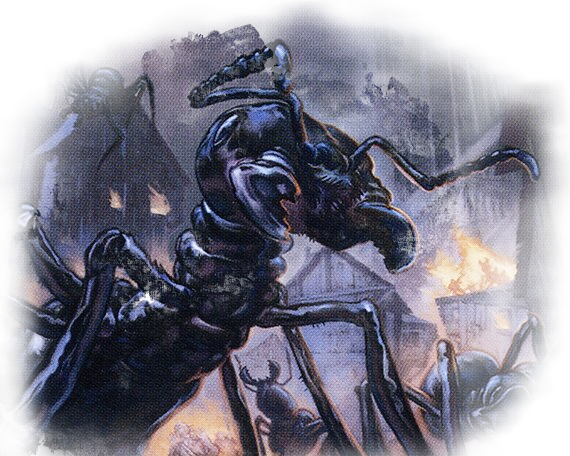
\includegraphics[width=\columnwidth -2em, height=190pt, keepaspectratio]{Soldier_Ant.png}};%
\end{tikzpicture}\end{center}\vspace*{-1.5cm}%
\addImageDBEntry{FleshgorgerAnt2}{Page \thepage}{Art}{https://gatherer.wizards.com/pages/Card/Details.aspx?multiverseid=534985}{Rise of the Ants MtG Art from Innistrad: Midnight Hunt}{Nicholas Gregory}%
% Monster stat block
\begin{DndMonster}[width=0.5\textwidth]{Fleshgorger Soldier Ant}
    \DndMonsterType{Large Monster, unaligned}

    % If you want to use commas in the key values, enclose the values in braces.
    \DndMonsterBasics[
        armor-class = {12 (Natural Armor)},
        hit-points  = {\DndDice{4d10+12}},
        speed       = {30 ft., burrow 25 ft., climb 25 ft.},
    ]

    \DndMonsterAbilityScores[
        str = 19,
        dex = 10,
        con = 17,
        int = 1,
        wis = 12,
        cha = 11,
    ]

    \DndMonsterDetails[
        %saving-throws = {Str +0, Dex +0, Con +0, Int +0, Wis +0, Cha +0},
        skills = {Acrobatics +8, Perception +3},
        %damage-vulnerabilities = {cold},
        %damage-resistances = {bludgeoning, piercing, and slashing from nonmagical attacks},
        %damage-immunities = {cold},
        senses = {blindsight 30ft., passive Perception 13},
        %condition-immunities = {frightened, poisoned},
        %languages = {-},
        challenge = 3,
    ]
    
    \DndMonsterAction{Powerful Build}
    The ant counts as one size larger for the purpose of determining its carrying capacity, the weight it can push, drag, or lift, and creatures it can grapple.
    
    \DndMonsterAction{Insect Climb}
    The ant can climb difficult surfaces without the need of performing ability checks.
    
    \DndMonsterAction{Hive Tactics}
    The ant has advantage on attack roles on creatures within 5 ft. of one of the ant's allies.
    
    \DndMonsterAction{Hive Mind}
    The ant is immune to being charmed or frightened.
	
	\DndMonsterSection{Actions}
	\DndMonsterAction{Multiattack}
	The Fleshgorger Ant can make a Hive Command, Bite Attack, and a Sting Attack on its turn.
	
	\DndMonsterAttack[
      name=Bite,
      distance=melee, % valid options are in the set {both,melee,ranged},
      %type=weapon, %valid options are in the set {weapon,spell}
      mod=+6,
      reach=5,
      %range=20/60,
      targets=one target,
      dmg=\DndDice{2d6 + 6},
      dmg-type=piercing,
      %plus-dmg=,
      %plus-dmg-type=,
      %or-dmg=,
      %or-dmg-when=,
      %extra=,
    ]
    
    \DndMonsterAttack[
      name=Sting,
      distance=melee, % valid options are in the set {both,melee,ranged},
      %type=weapon, %valid options are in the set {weapon,spell}
      mod=+6,
      reach=5,
      %range=20/60,
      targets=one target,
      dmg=\DndDice{1d10 + 4},
      dmg-type=piercing,
      %plus-dmg=,
      %plus-dmg-type=,
      %or-dmg=,
      %or-dmg-when=,
      extra={. Creatures must succed a DC 13 Constitution Saving Throw or take \DndDice{2d6} poison damage. On a successful save, it takes half damage},
    ]
    
    \DndMonsterAction{Hive Command}
    The Soldier Ant can command another visible ant within 30ft. of it to perform one of the following actions:
    \begin{itemize}
    		\item The ant can move up to its movement speed to make an attack against a creature within range using its reaction
    		\item The ant can use its reaction to repeat a saving throw against an effect.
    \end{itemize}
      
\end{DndMonster}

\noindent Giant Fleshgorger Ants organize themselves by having different specializations between its colony members. Worker Ants gather food and material and build up the ants mound and tunnel network. Soldier Ants deal with intruders and attackers and provide safety and security for the hive.\\
The Giant Ant Queen usually resides within the mound and is taken care by the colony members to ensure the survival of the colony.

% --------------------------------------------------------------------------------------------------- %
% ################################################################################################### %
% #-#-#-#-#-#-#-#-#-#-#-#-#-#-# Monster-Sheet with  full Banner-Graphic #-#-#-#-#-#-#-#-#-#-#-#-#-#-# %
% ################################################################################################### %
% --------------------------------------------------------------------------------------------------- %
\def\primarycolor{titlered}%
\def\secondarycolor{white}%
\MonsterBannerGraphic%
	{\entryfont{\shadowfy{Giant Ant Queen}}}% name of the monster to be displayed as header
	{section}% either section or chapter
	{247pt}% offset for the section header
	{325pt}% max height of the image
	{Queen_Ant.png}% image to be displayed as a banner
	{}% used for keepaspectratio for image ({} or {, keepaspectratio})
\addcontentsline{toc}{section}{Giant Ant Queen}
\addImageDBEntry{FleshgorgerAnt3}{Page \thepage}{Art}{https://www.artstation.com/artwork/EoGae}{Queen Ant}{Kim Sung Hwan}%
\vspace{13pt}
\entryfont \noindent \DndDropCapLine{T}he Giant Ant Queen is,\\
at least from the pers-\\
pective of an ant, con-\\
sidered a divine being, which the colony obeys without question. The colony provides her protection and nurishment while the queen itself is laying thousands of eggs, giving birth to the next generation of the colony.\\
A queen outside of her mound is a very rare sight and usually happens when the colony is on the move to a new territory.


% Monster stat block
\begin{DndMonster}[float*=b, width=\textwidth +8pt]{Giant Ant Queen}
    \vspace*{-17.5pt}\begin{multicols}{2}\DndMonsterType{Gragantuan Beast, unaligned}

    % If you want to use commas in the key values, enclose the values in braces.
    \DndMonsterBasics[
        armor-class = {16 (natural armor)},
        hit-points  = {\DndDice{7d20 + 28}},
        speed       = {30 ft., climb 25 ft., burrow 25 ft.},
    ]
    
    \renewcommand{\AbilityScoreSpacer}{~}

    \DndMonsterAbilityScores[
        str = 27,
        dex = 10,
        con = 18,
        int = 10,
        wis = 15,
        cha = 21,
    ]

    \DndMonsterDetails[
        %saving-throws = {Str +0, Dex +0, Con +0, Int +0, Wis +0, Cha +0},
        skills = {Acrobatics +13, Perception +7},
        %damage-vulnerabilities = {cold},
        %damage-resistances = {bludgeoning, piercing, and slashing from nonmagical attacks},
        %damage-immunities = {cold},
        senses = {blindsight 60ft, passive Perception 17},
        condition-immunities = {poisoned, charmed, frightened},
        %languages = {-},
        challenge = 12,
    ]
    
    \DndMonsterAction{Insect Climb}
    The Giant Ant Queen can climb difficult surfaces without the need of performing ability checks.
    
    \DndMonsterAction{Swarmlord}
    Ants that first enter or start their turn within 60 ft. of the Giant Ant Queen have advantage on attack rolls, ability checks, and saving throws of any kind.
    
    \DndMonsterAction{Swarm Frenzy}
    Ants that first enter or start their turn within 60 ft. of the Giant Ant Queen can perform an additional Bite attack during their Attack Action.
    
    \DndMonsterAction{Undying Servitude}
    Whenever an ant within 60 ft. of the Giant Ant Queen is reduced to 0 hitpoints, if it is not incapacitated, it can make a DC 10 Constitution Saving Throw regaining 1 hitpoint on a successful one.
    
    \DndMonsterAction{Hive Mind}
    The Giant Ant Queen is immune to being charmed or frightened.
	
	\vfill\eject\vspace*{-30pt}
	
	\DndMonsterSection{Actions}
	\DndMonsterAction{Multiattack}
	The Giant Ant Queen can make a Sting and a Bite attack each turn.
	
	\DndMonsterAttack[
      name=Bite,
      distance=melee, % valid options are in the set {both,melee,ranged},
      %type=weapon, %valid options are in the set {weapon,spell}
      mod=+11,
      reach=10,
      %range=20/60,
      targets=one target,
      dmg=\DndDice{4d10 + 7},
      dmg-type=piercing,
      %plus-dmg=,
      %plus-dmg-type=,
      %or-dmg=,
      %or-dmg-when=,
      extra={. The target must make a DC 18 Constitution Saving throw, taking \DndDice{2d6} poison damage on a failed save, or half as much on a successful one},
    ]
    
    \DndMonsterAttack[
      name=Sting,
      distance=melee, % valid options are in the set {both,melee,ranged},
      %type=weapon, %valid options are in the set {weapon,spell}
      mod=+11,
      reach=10,
      %range=20/60,
      targets=one target,
      dmg=\DndDice{4d4 + 7},
      dmg-type=piercing,
      %plus-dmg=,
      %plus-dmg-type=,
      %or-dmg=,
      %or-dmg-when=,
      extra={. The target must make a DC 18 Constitution Saving throw, taking \DndDice{8d6} poison damage on a failed save, or half as much on a successful one},
    ]
    
	\DndMonsterAction{Fury of the Swarm (Recharge 5-6)}
	Each ant within a 60 ft. radius of the Giant Ant Queen can use its reaction to move up to its movement speed and to make an Attack Action.
    
    \DndMonsterSection{Legendary Actions}
    The Giant Ant Queen can take 3 Legendary Actions, choosing from the options below. Only one Legendary Action can be used at a time and only at the end of a creature's turn. The Giant Ant Queen regains spent Legendary Actions at the start of its turn.
    \begin{DndMonsterLegendaryActions}
  		\DndMonsterLegendaryAction{Vitality Command}{The Giant Ant Queen can end one of the following effects on an ant it can see within 60 ft.: blinded, deafened, poisoned, stunned, paralyzed, or unconscious.}
  		\DndMonsterLegendaryAction{Battle Command}{The Giant Ant Queen can command one ant it can see within 60ft. to move up to its movement speed and make a Bite attack againsta creature of the queen's choice.}
  		\DndMonsterLegendaryAction{Burrow Shift (Costs 2 Actions)}{The Giant Ant Queen can travel burrow up to its full movement speed to a spot it can see. This movement does not provoke opportunity attacks.}
	\end{DndMonsterLegendaryActions}
\end{multicols}\end{DndMonster}

\vfill\eject\vspace*{8pt}

\subsection*{Soul of the Hive}
The very temperament and personality of the hive often reflects the nature of the queen. Some queens tend to be extremely aggressive resulting in deadly raids from ants. Others tend to be more passive and even tolerate the presence of other creatures like humanoids. Whenever a hive becomes dangerous or out of control, dealing with the queen is typically the most straight-forward solution.
	
	% Final Page
	\monstersLastPage{images/backcover_Mossdrip_Caverns.jpg}{0cm}{3cm}{height=\paperheight}{https://www.artstation.com/artwork/XBxBqD}{Overgrown Tomb}{Svetlin Velinov}{}
\end{document}